\documentclass{article}


% if you need to pass options to natbib, use, e.g.:
%     \PassOptionsToPackage{numbers, compress}{natbib}
% before loading neurips_2024


% ready for submission
\usepackage[nonatbib, preprint]{neurips_2024}


% to compile a preprint version, e.g., for submission to arXiv, add add the
% [preprint] option:
% \usepackage{iclr2025_conference,times}

\usepackage[utf8]{inputenc} % allow utf-8 input
\usepackage[T1]{fontenc}    % use 8-bit T1 fonts
\usepackage{hyperref}       % hyperlinks
\usepackage{url}            % simple URL typesetting
\usepackage{booktabs}       % professional-quality tables
\usepackage{amsfonts}       % blackboard math symbols
\usepackage{nicefrac}       % compact symbols for 1/2, etc.
\usepackage{microtype}      % microtypography

\hypersetup{
    colorlinks,
    linkcolor={red!50!black},
    citecolor={blue!50!black},
    urlcolor={blue!80!black}
}

\usepackage[
    backend=biber,
    citestyle=numeric,
    defernumbers=true,       % continuous numbering across bibliography sections
    giveninits=true,         % abbreviate first name
    doi=false,
    sortcites,
    natbib=true,
    isbn=false,
    uniquelist=false, % solves the problem of having two names and then et al.
    minnames=1,
    maxnames=2, % max number of names to display before switching to et al in main text
    maxbibnames=4, % max number of names to display before switching to et al in bibliogrtaphuy		    
    eprint=true,
    url=false,
]{biblatex}
\addbibresource{paperpile.bib}
\addbibresource{iclr2025_conference.bib}

\hypersetup{
    colorlinks,
    linkcolor={red!50!black},
    citecolor={blue!50!black},
    urlcolor={blue!80!black}
}


\newcommand{\draftonly}[1]{#1}
% \renewcommand{\draftonly}[1]{}  % uncomment to hide comments

\newcommand{\draftcomment}[1]{\draftonly{#1}}
\newcommand{\todo}[1]{\draftcomment{\textcolor{red}{\small [TODO: #1]}}}
\newcommand{\tsq}[1]{\draftcomment{\textcolor{orange}{\small [SQ: #1]}}}
\newcommand{\dam}[1]{\draftcomment{\textcolor{magenta}{\small [DAM: #1]}}}
\newcommand{\ns}[1]{\draftcomment{\textcolor{blue}{\small [NPS: #1]}}}


%%%%%%%%%%%%%%%%%%% SHARED PACKAGES %%%%%%%%%%%%%%%%%%%
%
% --- inline annotations
%
\newcommand{\red}[1]{{\color{red}#1}}
\newcommand{\todo}[1]{{\color{red}#1}}
\newcommand{\TODO}[1]{\textbf{\color{red}[TODO: #1]}}
% --- disable by uncommenting  
% \renewcommand{\TODO}[1]{}
% \renewcommand{\todo}[1]{#1}

\usepackage{xcolor}
\usepackage{graphicx}
\usepackage{booktabs}
\usepackage{amsmath} 
\usepackage{amsfonts}
\usepackage{amssymb}
\usepackage{multirow} 
\usepackage{makecell}
\newcommand{\shline}{\Xhline{1.1pt}} % Adjust thickness as desired 
%%%%%%%%%%%%%%%%%%%%%%%%%%%%%%%%%%%%%%%%%%%%%%%%%%%%%%%
% Working titles ranked in no particular order

% \title{The Fragility of Hierarchical Generalization:\\
% Minimal Data Requirements and the Power of Simplicity}

\title{Sometimes I am a Tree:
Data Drives Unstable Hierarchical Generalization}
% The \author macro works with any number of authors. There are two commands
% used to separate the names and addresses of multiple authors: \And and \AND.
%
% Using \And between authors leaves it to LaTeX to determine where to break the
% lines. Using \AND forces a line break at that point. So, if LaTeX puts 3 of 4
% authors names on the first line, and the last on the second line, try using
% \AND instead of \And before the third author name.



\author{
  Tian Qin \\
  Harvard University \\
  Cambridge, MA\\
   \texttt{tqin@g.harvard.edu} \\
  %% examples of more authors
   \And
  Naomi Saphra \\
  Harvard University \\
  Cambridge, MA\\
\texttt{nsaphra@fas.harvard.edu} \\
  \And
  David Alvarez-Melis \\
  Harvard University \& MSR \\
  Cambridge, MA\\
   \texttt{dam@seas.harvard.edu}  \\
}


\begin{document}

\maketitle
% keywords can be removed
% \keywords{First keyword \and Second keyword \and More}
% \input{sections/future_work}
\begin{abstract}
There is a widely-spread claim that GANs are difficult to train, and GAN architectures in the literature are littered with empirical tricks. We provide evidence against this claim and build a modern GAN baseline in a more principled manner. First, we derive a well-behaved regularized relativistic GAN loss that addresses issues of mode dropping and non-convergence that were previously tackled via a bag of ad-hoc tricks. We analyze our loss mathematically and prove that it admits local convergence guarantees, unlike most existing relativistic losses. Second, this loss allows us to discard all ad-hoc tricks and replace outdated backbones used in common GANs with modern architectures. Using StyleGAN2 as an example, we present a roadmap of simplification and modernization that results in a new minimalist baseline---\modelName (``Re-GAN''). Despite being simple, our approach surpasses StyleGAN2 on FFHQ, ImageNet, CIFAR, and Stacked MNIST datasets, and compares favorably against state-of-the-art GANs and diffusion models.\\
Code: \href{https://www.github.com/brownvc/R3GAN}{https://www.github.com/brownvc/R3GAN}
\end{abstract}
\section{Introduction}
\label{sec:intro}


Transformers, in particular decoder-only models (e.g.\ GPT~\citep{brown2020language}, Llama~\citep{touvron2023llama}) which process input sequences in a causal fashion, are one of the main drivers of modern deep learning's success.
Numerous approaches attempt to approximate the core attention layer to address its efficiency issues~\citep{tay2022efficient}, such as scaling quadratically in sequence length during training and requiring a cache of size linear in sequence length during autoregressive generation.
In parallel, a class of alternative sequence models, structured state-space models (SSMs), have emerged with linear scaling in sequence length during training and constant state size during generation.
They show strong performance on long-range tasks (e.g. S4~\citep{gu2022efficiently}) and recently matched or beat Transformers on language modeling (e.g. Mamba \citep{gu2023mamba}) at small to moderate scale.
However, the development of SSMs have appeared disjoint from the community's collective effort to improve Transformers, such as understanding them theoretically as well as optimizing them on modern hardware.
As a result, it is more difficult to understand and experiment with SSMs compared to Transformers, and it remains challenging to train SSMs as efficiently as Transformers from both an algorithmic and systems perspective.


Our main goal is to develop a rich body of theoretical connections between structured SSMs and variants of attention.
This will allow us to transfer algorithmic and systems optimizations originally developed for Transformers to SSMs, towards the goal of building foundation models that perform better than Transformers while scaling more efficiently in sequence length.
A milestone contribution in this direction was the \textbf{Linear Attention (LA)} framework \citep{katharopoulos2020transformers},
which derived a connection between autoregressive attention and linear RNNs
by showing the equivalence between ``dual forms'' of quadratic kernelized attention and a particular linear recurrence.
This duality allows new capabilities such as the ability to have both efficient parallelizable training and efficient autoregressive inference.
In the same spirit, this paper provides multiple viewpoints connecting linear-complexity SSMs with quadratic-complexity forms to combine the strengths of SSMs and attention.%
\footnote{Technically speaking, these connections only relate to certain flavors of attention; the title of this paper is an homage to \citet{katharopoulos2020transformers} which first showed that ``Transformers are RNNs''.}

\iftoggle{arxiv}{
\begin{wrapfigure}{R}{0.48\linewidth}
  \begin{center}
    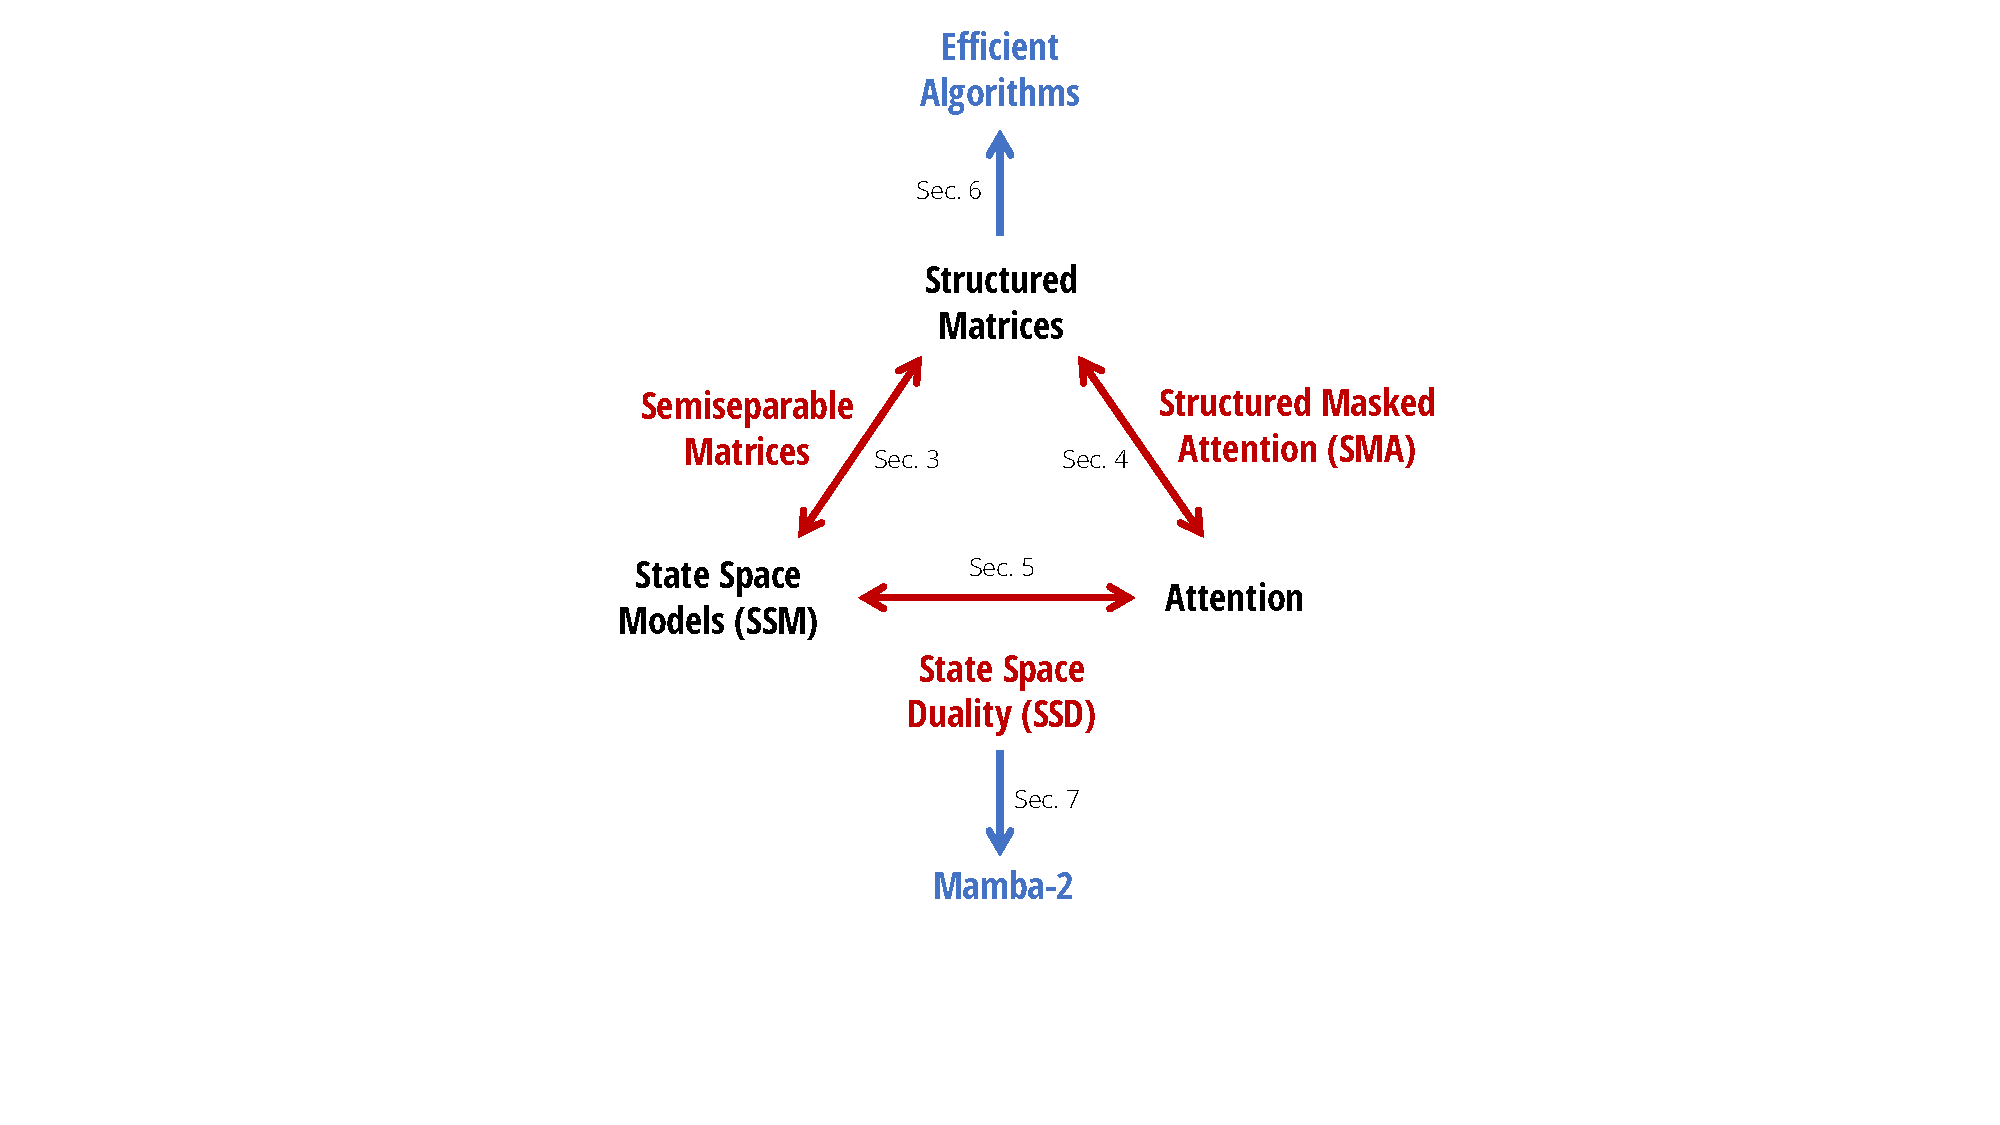
\includegraphics[width=\linewidth]{fig/ssd_roadmap.pdf}
  \end{center}
  \caption{
    (\textbf{Structured State-Space Duality}.)
    This paper fleshes out the relationship between state space models and attention through the bridge of structured matrices.
  }
  \label{fig:roadmap}
\end{wrapfigure}
}{}

\para{State Space Duality.}
Our framework connecting structured SSMs and variants of attention, which we call \textbf{structured state space duality} (SSD),
is made through the abstractions of \textbf{structured matrices}:
matrices with subquadratic parameters and multiplication complexity.
We develop two broad frameworks for representing sequence models, one as matrix transformations and one as tensor contractions, which each reveal different perspectives of the duality.
Our technical contributions include:
\begin{itemize}[leftmargin=*,itemsep=0pt,topsep=0pt]
  \item We show an equivalence between state space models and a well-studied family of structured matrices called \textbf{semiseparable matrices}\iftoggle{arxiv}{ (\cref{sec:ssm})}{}.
    This connection is at the heart our framework, revealing new properties and algorithms for SSMs. A central message of this paper is that \emph{different methods of computing state space models can be reframed as various matrix multiplication algorithms on structured matrices}.
  \item We significantly improve the theory of linear attention~\citep{katharopoulos2020transformers}.
    We first provide an incisive proof of its recurrent form through the language of tensor contractions, and then generalize it to a new family of \textbf{structured masked attention (SMA)}\iftoggle{arxiv}{ (\cref{sec:attention})}{}.
  \item We connect SSMs and SMA, showing that they have a large intersection that are duals of each other, possessing both SSM-like linear and attention-like quadratic forms\iftoggle{arxiv}{ (\cref{sec:ssd})}{}.
    \iftoggle{arxiv}{We also prove that any kernel attention method possessing a fast recurrent form must be an SSM.}{}
\end{itemize}


Beyond its intrinsic theoretical value, our framework opens up a broad set of directions for understanding and improving sequence models.

\para{Efficient Algorithms.}
First and most importantly, our framework exposes new efficient and easily-implementable algorithms for computing SSMs\iftoggle{arxiv}{ (\cref{sec:efficient})}{}.
We introduce a new \textbf{SSD algorithm}, based on block decompositions of semiseparable matrices, that takes advantage of both the linear SSM recurrence and quadratic dual form, obtaining optimal tradeoffs on all main efficiency axes (e.g. training and inference compute, memory usage, and ability to leverage matrix multiplication units on modern hardware).
A dedicated implementation of SSD is $2-8\times$ faster than the optimized selective scan implementation of Mamba, while simultaneously allowing for much larger recurrent state sizes ($8\times$ the size of Mamba or even higher, with minimal slowdown).
SSD is highly competitive with optimized implementations of softmax attention (FlashAttention-2~\citep{dao2023flashattention2}), crossing over at sequence length 2K and 6$\times$ faster at sequence length 16K.


\iftoggle{arxiv}{
\para{Architecture Design.}
One major obstacle to adopting new architectures such as SSMs is the ecosystem tailored to Transformers, such as hardware-efficient optimization and parallelism techniques for large-scale training.
Our framework allows using established conventions and techniques for attention to build a vocabulary of architecture design choices for SSMs, and further improve them (\cref{sec:architecture}).
For example, we introduce the analog of heads from multi-head attention (MHA) to SSMs.
We show that the Mamba architecture is a \textbf{multi-input SSM (MIS)} that turns out to be analogous to \textbf{multi-value attention (MVA)}, and compare other variants of Mamba with different head structures.

We also use these ideas to make slight modifications to the Mamba block, which allows tensor parallelism to be implemented (e.g. in the style of Megatron~\citep{shoeybi2019megatron}).
The main ideas include introducing grouped-value attention (GVA) head structure, and moving all data-dependent projections to occur in parallel at the beginning of the block.


}{
  \para{Mamba-2.}
  Additionally, inspired by the connection between SSMs and Transformers, we slightly modify the neural network architecture of Mamba by moving all data-dependent projections to occur in parallel at the beginning of the block. %
}
The combination of the modified parallel Mamba block, together with using SSD as the inner SSM layer, results in the \textbf{Mamba-2} architecture.
We investigate Chinchilla scaling laws for Mamba-2 in the same setting as Mamba, finding that it Pareto dominates Mamba and Transformer++ in both perplexity and wall-clock time.
We additionally train a family of Mamba-2 models at varying sizes on the Pile, showing that it matches or outperforms Mamba and open source Transformers on standard downstream evaluations.
For example, Mamba-2 with 2.7B parameters trained on 300B tokens on the Pile outperforms Mamba-2.8B, Pythia-2.8B and even Pythia-6.9B trained on the same dataset.

\iftoggle{arxiv}{
\paragraph{Systems Optimizations.}
The SSD framework connects SSMs and Transformers, allowing us to leverage a rich body of work on systems optimizations developed for Transformers~(\cref{sec:systems}).
\begin{itemize}[leftmargin=*,itemsep=0pt,topsep=0pt]
  \item For example, Tensor Parallelism (TP) is an important model parallelism technique to train large Transformer models by splitting each layer across GPUs on the same node.
    We design Mamba-2 to be TP-friendly, reducing the number of synchronization point per block by half.
  \item For very long sequences whose activations do not fit on one device, sequence parallelism has been developed for the attention blocks.
    We describe how to train SSMs in general and Mamba-2 in particular with sequence parallelism, by passing the recurrent states between devices.
  \item For finetuning with examples of different lengths, for best efficiency, Transformer requires sophisticated techniques to remove padding tokens and perform attention on variable length sequences.
    We show how Mamba-2 can be trained with variable sequence lengths efficiently, requiring no padding tokens.
\end{itemize}
}{}

\cref{sec:experiments} empirically validates Mamba-2 on language modeling, training efficiency, and a difficult multi-query associative recall task~\citep{arora2024simple}.
Finally, in \cref{sec:related}, we provide an extended related work and discuss potential research directions opened up by our framework.

Model code and pre-trained checkpoints are open-sourced at \url{https://github.com/state-spaces/mamba}.






\section{Background}
Our extended literature review in Appendix \ref{appdx:related} expands on the following background overview.


\subsection{Syntax and Hierarchical Generalization}
\label{sec:syntax_related}
% \paragraph{Syntax and Hierarchical Generalization}
\citet{McCoy2018-uv} first used the question formation task to study hierarchical generalization in neural networks, showing that attention mechanisms improved generalization performance in RNNs. Later, \citet{McCoy2020-pj} found that tree-structured architectures consistently induce hierarchical generalization. \citet{Petty2021-pe} and \citet{Mueller2022-rm} further concluded that  transformers tend to generalize linearly. This view was challenged by \citet{Murty2023-xp}, who attributed the failure of prior attempts to insufficient training, demonstrating that decoder-only transformers can generalize hierarchically, but only after in-distribution performance has plateaued. They named this transition from surface-level heuristics to hierarchical generalization structural grokking. Expanding on their findings, \citet{Ahuja2024-ul} showed that models only generalize hierarchically when trained on a language modeling objective. All of this prior work attributed hierarchical inductive bias to model architecture or objective, whereas our study highlights the impact data. 
While previous work observed some inconsistency across seeds \citep{McCoy2018-uv, McCoyUnknown-uy}, we further characterize the specific distributions produced by this inconsistency. 


\subsection{Training Dynamics and Grokking}
During \textit{grokking}, a neural network suddenly generalizes to a test set long after it has overfitted to its training data. \citet{Power2022-hz} first observed this phenomenon in simple arithmetic tasks. 
This classic grokking is different from our main focus---\textit{structural grokking} \citep{Murty2023-xp}. In classic grokking, the model transitions from memorization to generalization, allowing it to achieve non-trivial performance on unseen data from the same distribution as the train set. In structural grokking, a model transitions from the simple linear rule to the hierarchical rule, leading to non-trivial performance on OOD data. However, our findings also relate to classic grokking through our study of data diversity and memorization. 

\citet{Zhu2024-nz} studied the role of data and finds that grokking only occurs when training set is sufficiently large, and thus more diverse. \citet{Berlot-Attwell2023-qx} studied how data diversity leads to OOD compositional generalization in multimodal models and 
\citet{Lubana2024-ed} showed that diversity also induces compositional behaviors late in LM training.
\citet{Liu2022-mj} showed grokking can be induced by forcing a specific weight norm, a measurement of model---not data---complexity. 
\citet{Huang2024-aw} and \citet{Varma2023-iq} have shown that during training, different circuit compete and data and model size can lead to different competition and training dynamics. Circuit competitions also shape other phase transitions, such as transient in-context learning \citep{Park2024-ri}.
% While these works primarily study training dynamics, our findings highlight that this competition can also lead to inconsistent outcomes when training converges.
% We unify these threads in the existing grokking literature by characterizing the unstable regime in both data diversity and data complexity, connecting training stability with consistency under random seeds.


\subsection{Random Variation} 
Although choices like hyperparameters, architecture, and optimizer all shape model outcomes, training remains inherently stochastic. Models are sensitive to random initialization and the order of training examples \cite{Dodge2020-pb}. Several studies \citep{Zhou2020-xt, D-Amour2022-tl, Naik2018-og} have reported significant performance difference across random seeds. \citet{Zhou2020-xt} further observed that on Natural Language Inference (NLI) tasks, OOD instability is observed throughout training. We investigate the source of these training inconsistencies and link them more precisely to characteristics of the training data. 




\subsection{Data Augmentation in NLP}
The problem of domain adaptation and OOD robustness is well established in NLP \citep{blitzer-etal-2007-biographies,daume-iii-2007-frustratingly,hendrycks2020pretrained}.
Existing work on improving generalization has focused on data augmentation, where synthetically generated training examples are used to augment an existing dataset.
It is hypothesized that these examples induce robustness to local perturbations, which has been shown to be effective in semi-supervised and self-supervised settings \citep{bachman2014learning,szegedy2014intriguing, sajjadi2016regularization}.

Existing task-specific methods \citep{kafle-etal-2017-data} and word-level methods \citep{zhang2015character, xie2017data, wei-zou-2019-eda} are based on human-designed heuristics.
Back-translation from or through another language has been applied in the context of machine translation \citep{sennrich2016improving}, question answering \citep{wei2018fast}, and consistency training \citep{xie2019unsupervised}.
More recent work has used word embeddings \citep{wangyang2015thats} and LSTM language models \citep{fadaee2017data} to perform word replacement.
Other methods focus on fine-tuning contextual language models \citep{kobayashi-2018-contextual,wu2019conditional,kumar20202data} or large generative models \citep{lambada,yang2020g-daug,kumar20202data} to generate synthetic examples.

\subsection{VRM and the Manifold Assumption}
Vicinal Risk Minimization (VRM) \citep{vicinal200olivier} formalizes data augmentation as enlarging the training set support by drawing samples from a \textit{vicinity} of existing training examples.
Typically the vicinity of a training example is defined using dataset-dependent heuristics.
For example, in computer vision, examples are generated using scale augmentation \citep{simonyan2014very}, color augmentation \citep{krizhevsky2012imagenet}, and translation and rotation \citep{Simard1998}.

The \textit{manifold assumption} states that high dimensional data concentrates around a low-dimensional manifold \citep{chapelle2006semi}.
This assumption allows us to define the vicinity of a training example as its \textit{manifold neighborhood}, the portion of the neighborhood that lies on the data manifold.
Recent methods have used the manifold assumption to improve robustness by moving examples towards a decision boundary \citep{kanbak2018geometric}, generating adversarial examples \cite{szegedy2014intriguing,miyato2017virtual}, interpolating between pairs of examples \citep{zhang2018mixup}, or finding affine transforms \citep{paschali2019data}.

\begin{figure}[t!]
\centering
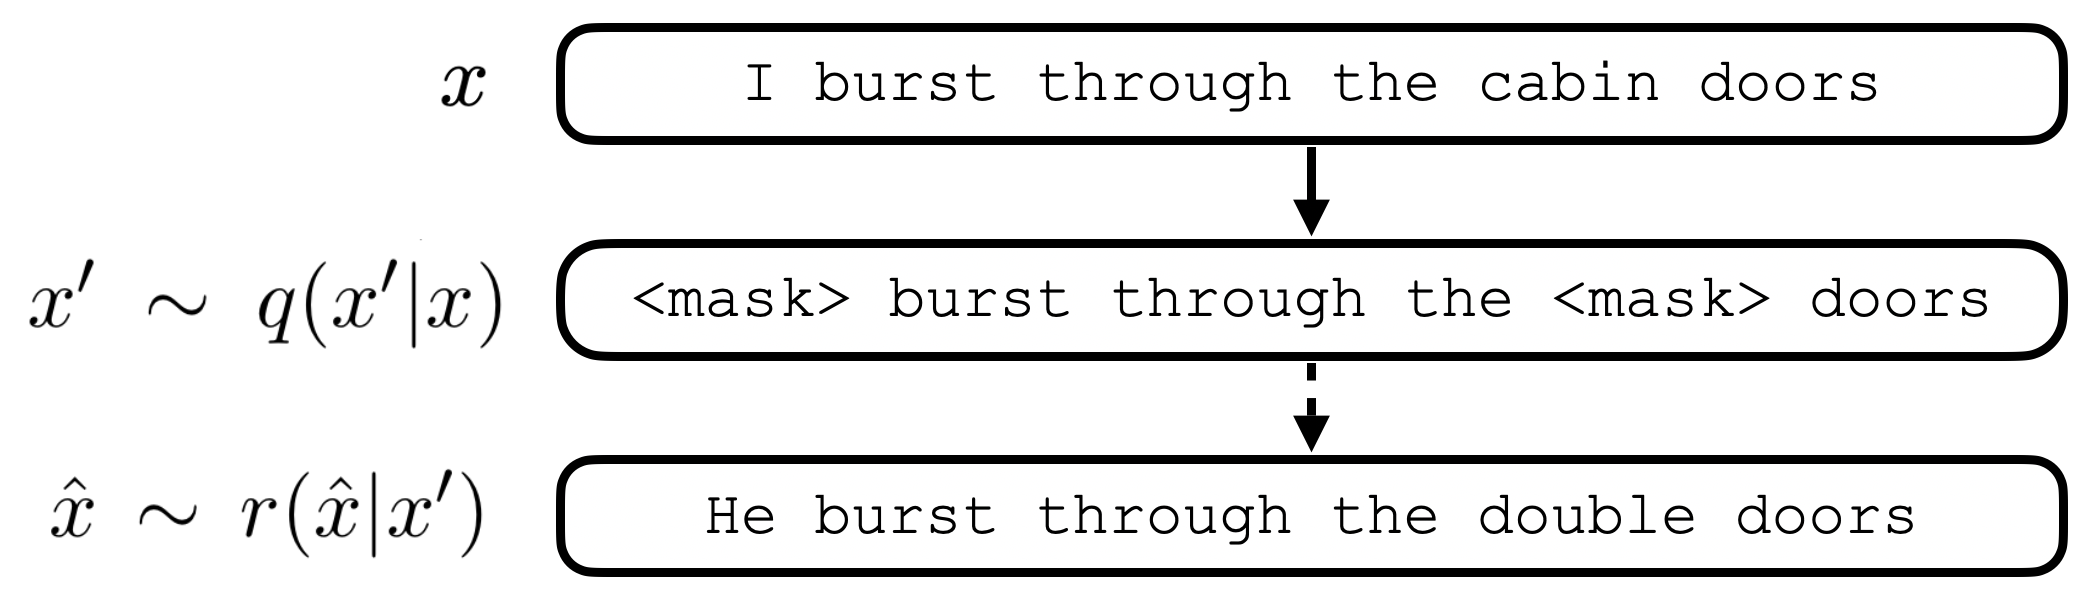
\includegraphics[scale=0.21]{img/bert_dae.png}
\caption{To sample from an MLM DAE, we apply the MLM corruption $q$ to the original sentence then reconstruct the corrupted sentence using our DAE $r$.}
\label{fig:dae_sampling}
\end{figure}

\subsection{Sampling from Denoising Autoencoders}
A denoising autoencoder (DAE) is an autoencoder trained to reconstruct a clean input $x$ from a stochastically corrupted one $x'\sim q(x'|x)$ by learning a conditional distribution $P_\theta (x| x')$ \citep{vincent2008extracting}.
We can sample from a DAE by successively corrupting and reconstructing an input using the following pseudo-Gibbs Markov chain: $x_t' \sim q(x'|x_{t-1})$, $x_t \sim P_\theta(x|x'_t).$
\comment{
\begin{align*}
    x_t' &\sim q(x'|x_{t-1})\\
    x_t &\sim P_\theta(x|x'_t) 
\end{align*}
}
As the number of training examples increases, the asymptotic distribution $\pi_n(x)$ of the generated samples approximate the true data-generating distribution $P(x)$ \citep{bengio2013generalized}.
This corruption-reconstruction process allows for sampling directly along the manifold that $P(x)$ concentrates on.

\subsection{Masked Language Models}
Recent advances in unsupervised representation learning for natural language have relied on pre-training models on a \textit{masked language modeling} (MLM) objective \citep{devlin2018, liu2019roberta}.
In the MLM objective, a percentage of the input tokens are randomly corrupted and the model is asked to reconstruct the original token given its left and right context in the corrupted sentence.
We use MLMs as DAEs \citep{lewis2019bart} to sample from the underlying natural language distribution by corrupting and reconstructing inputs (Figure \ref{fig:dae_sampling}).

\section{Data Design for creative writing evaluation}

\begin{table*}
\def\arraystretch{1.35}
\small
\centering
\begin{tabular}{|l|l|}
\hline
Story                                    & Plot                                                                                                                                                                                                                                                                                                                                                                                                                                                                                                                                   \\ \hline
\href{https://www.newyorker.com/books/flash-fiction/a-triangle}{A Triangle}                               & \begin{tabular}[c]{@{}l@{}}An observer becomes entranced by a seemingly ordinary couple on the street, follows them home,\\ and then watches them from  outside in the rising floodwaters, drawing an eerie connection \\ between the woman and a discarded, burned chair they'd noticed earlier.\end{tabular}                                                                                                                                                                    \\ \hline\hline
\href{https://www.newyorker.com/books/flash-fiction/barbara-detroit-1966}{Barbara,Detroit,1996 }                    & \begin{tabular}[c]{@{}l@{}}On February 12, 1966, a heavily pregnant woman named Barbara experienced a shocking incident in her\\ synagogue in Southfield, Detroit, where a young man shot and killed the renowned Rabbi Adler before\\ turning the gun on himself, and though Barbara tried to reach the shooter, she was swept away by the\\ fleeing crowd.\end{tabular}                                                                              \\ \hline\hline
\href{https://www.newyorker.com/books/flash-fiction/beyond-nature}{Beyond Nature}                           & \begin{tabular}[c]{@{}l@{}}A solitary man walking in a remote mountainous region comes across a car crash, and stays by the side\\ of the lifeless female victim, narrating stories of his past and reflecting on the impermanence of \\events and life itself, while awaiting emergency services amidst the looming presence of wilderness.\end{tabular}                                                                                                                \\ \hline\hline
\href{https://www.newyorker.com/books/flash-fiction/certain-european-movies}{Certain European Movies}                  & \begin{tabular}[c]{@{}l@{}}Two individuals, who are at a residency together, navigate the complexity of their ephemeral relationship \\during their final beach trip, framed by misadventures, subtle tensions, unspoken desires, and \\looming departures.\end{tabular}                                                                                                                                                                                   \\ \hline\hline
\href{https://www.newyorker.com/books/flash-fiction/keys}{Keys}                                     & \begin{tabular}[c]{@{}l@{}}Daniel, struggling with recurring dreams of his ex-wife Rachel and a mysterious unused flat, eventually \\discusses them with his current partner Isabel, sparking various reflections and conversations about their\\ past relationships, until a real-life discovery of old keys triggers a nostalgic memory and helps him find a\\ way to reconnect with his present relationship through canoeing.\end{tabular}                                     \\ \hline\hline
\href{https://www.newyorker.com/books/flash-fiction/listening-for-the-click}{Listening For the Click}                  & \begin{tabular}[c]{@{}l@{}}Navigating a complex social landscape, the protagonist experiences a series of complex relationships \\and emotional turmoil in a student  environment, and engages in self-discovery and self-reflection as she\\ interacts with the characters Carl, Martin, Lizzy, and Johan, resulting in a journey of introspection, betrayal,\\ love, and personal growth.\end{tabular}                                                          \\ \hline\hline
\href{https://www.newyorker.com/magazine/2023/05/15/maintenance-hvidovre-fiction-olga-ravn}{Maintenance, Hvidovre}                   & \begin{tabular}[c]{@{}l@{}}A woman experiences a disorienting night in a maternity ward where she encounters other similarly \\disoriented new mothers, leading to an uncanny mix-up where she leaves the hospital with a baby that she \\realizes is not her own, yet accepts the situation with an inexplicable sense of happiness.\end{tabular}                                                                                                  \\ \hline\hline
\href{https://www.newyorker.com/magazine/2022/11/14/returns}{Returns}                                  & \begin{tabular}[c]{@{}l@{}}The narrator visits their elderly mother in her small town, spending a day with her that is filled with \\nostalgia, conversation, and old habits, only to return a month later after her hospitalization due to\\ a sunstroke, finding remnants of their last visit.\end{tabular}                                                                                                                                                                      \\ \hline\hline
\href{https://www.newyorker.com/books/flash-fiction/the-facade-renovation-thats-going-well}{\begin{tabular}[c]{@{}l@{}}The Facade Renovation That’s \\Going Well\end{tabular}} & \begin{tabular}[c]{@{}l@{}}An academic faculty housed in a building with a critical waterproofing layer missing experiences a series\\ of disruptive and problematic construction repairs, causing tension, inconvenience, and health concerns\\ among the tenants, but ultimately leading to resignation and endurance in hopes of better future\\ circumstances.\end{tabular}                                                        \\ \hline\hline
\href{https://www.newyorker.com/books/flash-fiction/the-kingdom-that-failed}{The Kingdom That Failed}                  & \begin{tabular}[c]{@{}l@{}}The narrator recounts their college friendship with the seemingly flawless Q, and after a decade apart, \\they accidentally cross paths at a pool, where the narrator anonymously observes Q's failed attempt to \\let down a woman about a work-related issue, demonstrating that Q, too, has his share of difficulties.\end{tabular}                                                                                                \\ \hline\hline
\href{https://www.newyorker.com/magazine/2022/06/13/trash }{Trash}                                    & \begin{tabular}[c]{@{}l@{}}A woman unexpectedly marries the son of a successful, ambitious woman named Miss Emily, finding both \\acceptance and critique from her mother-in-law as she navigates this new relationship and confronts the \\stark contrasts between her  former life as a supermarket cashier and her new life as part of a well-off family.\end{tabular}                                                                                                            \\ \hline\hline
\href{https://www.newyorker.com/culture/personal-history/the-last-dance-with-my-dad}{The Last Dance with my Dad}               & \begin{tabular}[c]{@{}l@{}}A young teenager recounts her experiences of fitting into her father's gay lifestyle, highlighted by a\\ seven-day cruise with hundreds of gay men, where she  experienced acceptance and connection, had her\\ first genuine interaction with a  boy, and shared a last dance with her terminally ill father.\end{tabular}                                                                                                       \\ \hline
\end{tabular}
\vspace{2ex}
\caption{\label{teststories} Expert-written short stories from the New Yorker along with their human-verified GPT4 generated summary as plots that are included as part of our test data for Creativity Evaluation}
\end{table*}


Large Language models have been shown to automatically generate long and coherent stories \cite{yang2022doc,yang2022re3} as well as act as collaborators for creative writing \cite{yuan2022wordcraft,ippolito2022creative,mirowski2023cowriting}. However, there have been fewer studies showing how LLM-generated stories differ from expert written stories on metrics that are more fine-grained and objective.Our investigation involves an analysis of a dozen narratives authored by humans, as detailed in Table \ref{teststories}, extracted from The New Yorker. These narratives span a variety of esteemed authors, ranging from \textit{Haruki Murakami} to Nobel laureate \textit{Annie Ernaux}. The protocol for our human assessment incorporates two primary components: 

\begin{itemize}[leftmargin=*]
    \itemsep0em 
    \item Absolute evaluation of creative writing, disregarding whether it has been composed by a human or a LLM
    \item Relative evaluation for discerning whether a story has been produced by a human or an LLM( Turing Test).
\end{itemize}


\begin{figure*}
\centering
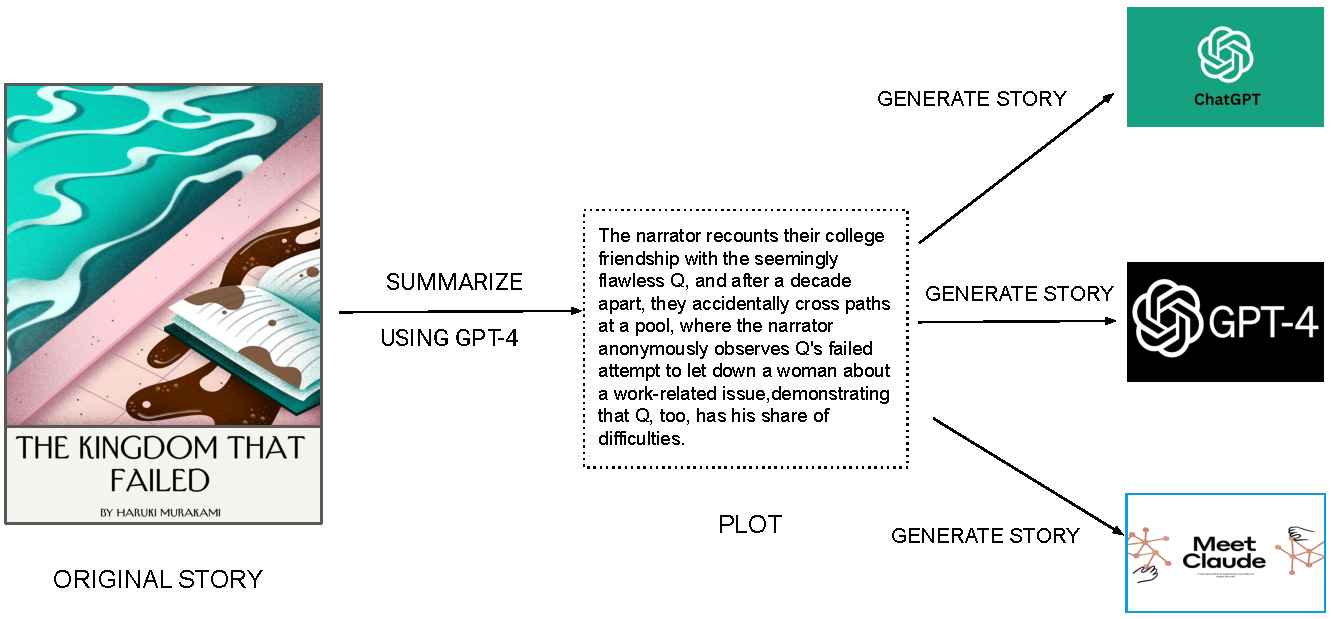
\includegraphics[width=\textwidth]{figures/datapipeline.pdf}
\caption{\label{datapipeline}Pipeline showing how our test set is created for evaluation. For each human-written original NewYorker story, we generate 3 stories from one LLM each, based on the plot of the original story. The plot is a single-sentence summary of the original story automatically generated by GPT-4 and verified by humans.}
\end{figure*}


In order to allow relative evaluation each human-authored narrative is summarized into a single-sentence plot, which is further verified by human evaluators. We then prompt three LLMs: GPT3.5, GPT4, and Claude, to generate a story conditioned on this plot summary. This yields a total of 48 short narratives for absolute evaluation (12 human written; 36 LLM written). Following this, we assign four stories centered around a single plot (one human-authored versus three LLM-authored) to a singular cluster, culminating in a total of 12 clusters. The methodology for creating an individual cluster is illustrated in Figure \ref{datapipeline}. The decision to employ human-authored plot summaries to prompt the LLMs is informed by the recognized shortfall of LLMs in their ability to devise original plotlines, as highlighted in previous research \cite{ippolito2022creative}. Furthermore, the utilization of multiple stories derived from the same plot enables experts to concentrate specifically on the human aspects of creative writing, and enhances their capacity to distinguish human-generated content from AI-produced ones.

In our quest to prevent straightforward parameters from differentiating between stories penned by human authors versus those produced by artificial intelligence (AI), we implemented strategies to ensure comparable story lengths across both classes. Initial experimentation revealed a notable discrepancy: Large Language Models (LLMs), when instructed to generate narratives of a predetermined word count, consistently underperformed, resulting in stories that were invariably more concise than intended. To address this inconsistency, we employed an iterative mechanism, prompting the LLM to iteratively rewrite the initial story until the divergence in word count between the AI-generated and human-composed story was less than 200 for every cluster. Table \ref{promptstory} (Row1) shows the original story prompt, while (Row2) illustrates the subsequent instruction to rewrite the story. We start the iterative process by prompting the LLM to expand the initially generated story. This cycle continued until the narrative length reached the pre-specified threshold or when the iteration count exceeded twenty ($loop\_count > $20). This methodology ensured the creation of AI-written stories with length characteristics more akin to those produced by human authors.

\begin{figure*}
\small
\centering
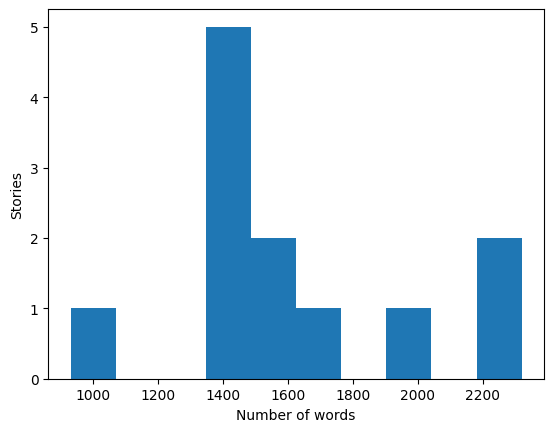
\includegraphics[width=\textwidth]{figures/length.png}
\caption{\label{length} Distribution of word count amongst the stories in our test set}
\end{figure*}


\begin{table}[]
\centering
\small
\def\arraystretch{1.35}
\begin{tabular}{|l|}
\hline
\begin{tabular}[c]{@{}l@{}}Write a New Yorker-style story given the plot below. Make sure it is atleast \textbf{\color{blue}\{\{word\_count\}\}} words. Directly start with the\\ story, do not say things like `Here's the story {[}...{]}:\end{tabular}                                                                                                                                                                                            \\ \hline\hline
\begin{tabular}[c]{@{}l@{}}You wrote the story I gave you below. I requested a story with \textbf{\color{blue}\{\{word\_count\}\}} words, but the story only has\\ \textbf{\color{blue}\{\{current\_word\_count\}\}} words. Can you rewrite the story to make it longer, and closer to the \textbf{\color{blue}\{\{word\_count\}\}} word target\\ I gave you. Directly start with the story, do not say things like `Here's the story {[}...{]}:`\\ \\ Current story: \{\{story\}\}\end{tabular} \\ \hline
\end{tabular}
\vspace{2ex}
\caption{\label{promptstory}Prompt to write the initial story (Row1) vs Prompt to rewrite the initial story to be longer. word\_count represents the number of words in the human written story on a given plot (P) while current\_word\_count represents the number of words in the LLM generated story on the same plot (P)}
\vspace{-7ex}
\end{table}

%     
%     \begin{subfigure}[b]{1.0\textwidth}
%          \centering
%          
\section{Training Stabilizes if a Model Commits to a Rule}
\label{sec:stability}
Why do some runs fail to generalize hierarchically even when trained on hierarchy-inducing data? In this section, we will show that these failures are consequences of training instability; models only stabilize OOD if they commit to a general rule, whether it is the hierarchical or linear rule. Some random seeds fail to stabilize regardless of our training set composition.


\subsection{Instability During Training} 
\label{sec:tv_def}
When training models on both QF and TI tasks, some random seeds lead to highly unstable OOD behavior, with OOD generalization accuracy oscillating during training (see Appendix \ref{appdx:training_instabilty} for example training curves). We measure instability across training time using \textbf{total variation} (TV). Specifically, we checkpoint the model every 2K steps and measure the generalization accuracy $\mathrm{Acc}_t$ at each checkpoint timestep $t \in T$. The total variation is defined as: 
\begin{wrapfigure}[]{r}{0.4\textwidth}
    \centering
    \vspace{5mm}
    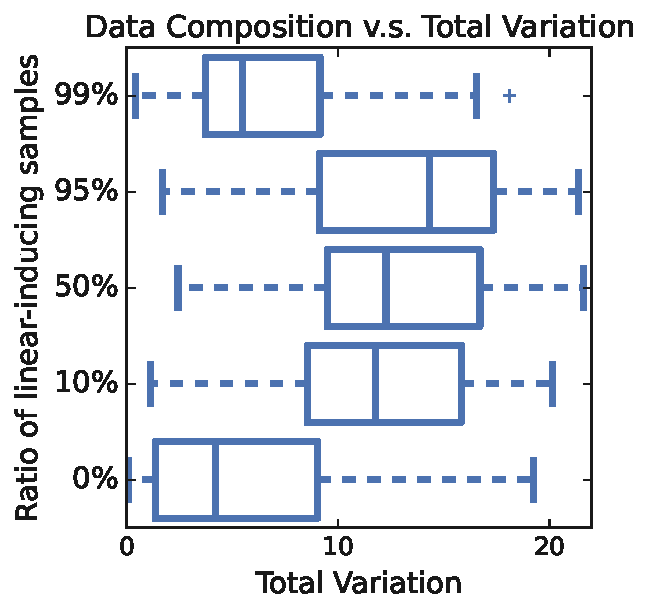
\includegraphics[width=0.85\linewidth]{figures/total_variation_box.pdf}
    \caption{\textbf{Training is unstable when different subsets of data compete.} Balanced mixtures of right-branching and center-embedded sentences have higher total variation than mixtures dominated by one or the other subset.}
    \vspace{-15mm}
    \label{fig:data_drives_inconsistency}
\end{wrapfigure}
\begin{align}
    \text{Total Variation (TV)} = 
    \frac{1}{|T|} \sum_{t \in T} 
    \left| \mathrm{Acc}_t - \mathrm{Acc}_{t-1} \right|
\end{align}

\subsection{Training Stability Ties to Rule Commitment}
\label{sec:intra_inter}

We now demonstrate that stable OOD behavior is associated with rule commitment. We construct QF training datasets with different proportions of hierarchy-inducing (i.e., center-embedded) and linearity-inducing (i.e., right-branching) declaration examples, while keeping all question examples from the original training set. Further details on the dataset can be found in Appendix~\ref{sec:simple_mixin}.


Figure \ref{fig:data_drives_inconsistency} shows the relationship between data homogeneity and training stability. When the training data is dominated by either linearity-inducing  (99\% linear) or hierarchy-inducing  (0\% linear) examples, more random seeds lead to stable OOD curves. When the training data is a heterogeneous mix instead, potential rules compete, leading to a higher proportion of unstable training runs.

By controlling for training instability, we reveal that generalization behavior is clustered and highly bimodal across random seeds. As shown in Figure \ref{fig:intra_inter_variance}, regardless of the data mix, the final generalization accuracy for all stable models is either $100\%$ or $0\%$---that is, stable models always commit to a systematic rule. 
While either rule can be implemented by a stable model, training data composition determines how likely a run is to stabilize in any rule and whether that rule is likely to be hierarchical or linear. 
Interestingly, when the data is heterogeneous (e.g., 10\% of examples are linearity-inducing right-branching sequences), the final generalization accuracy for stable runs is bimodally distributed, clustering around $100\%$ or $0\%$. 
 In fact, the horseshoe-shaped curves in Figure \ref{fig:intra_inter_variance} illustrate that the less stable a training run is, the less systematic the model tends to be in its OOD rules. 

\begin{figure}[t!]
    \centering
    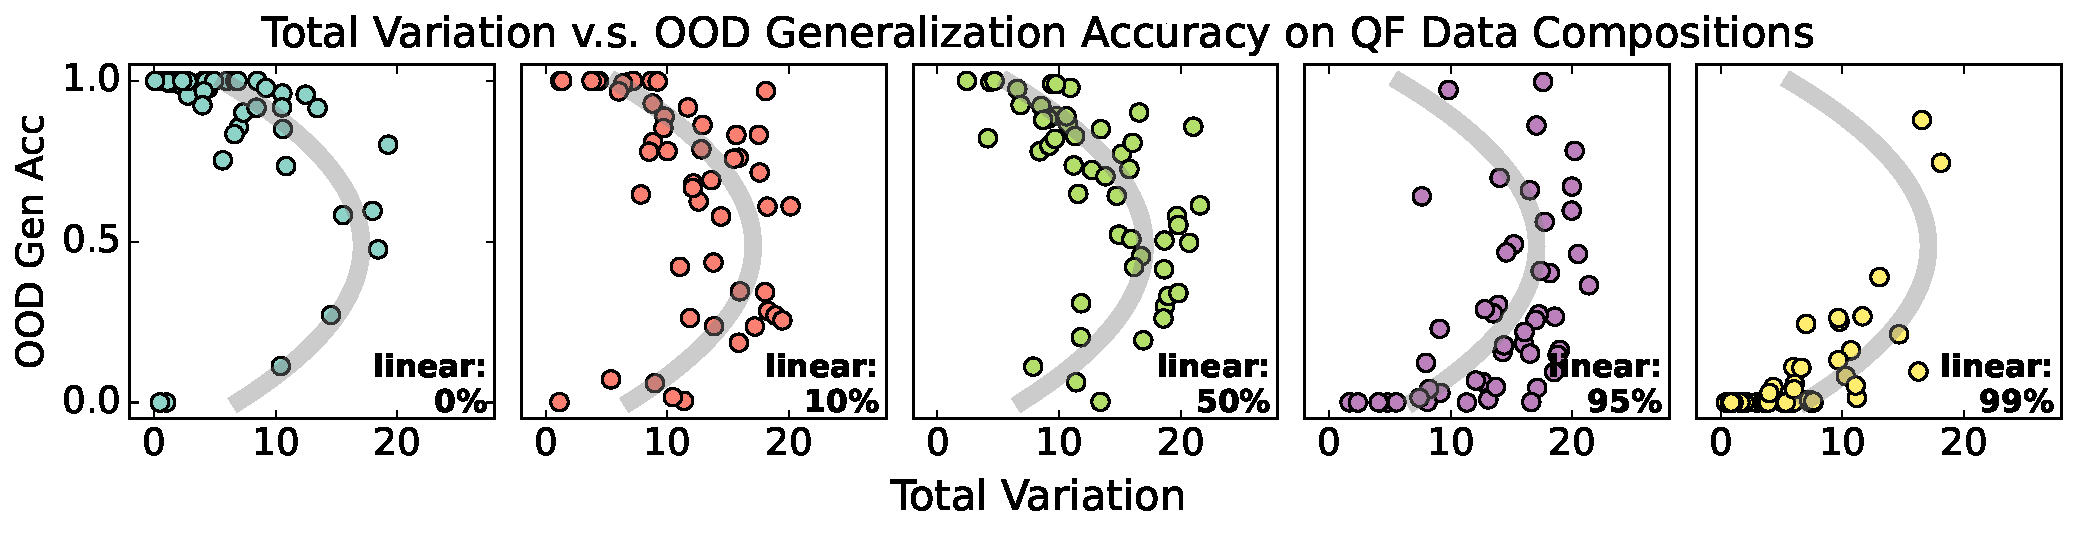
\includegraphics[width=1.0\linewidth]{figures/intra_inter_inconsistency_D270.pdf}
    \caption{\textbf{Training stability vs. final generalization accuracy for QF task.} OOD behavior stabilizes during training if a model commits to a general rule. By mixing data that induces the linear and hierarchical rules, we can create conditions that allow models to stabilize in either rule. ``Linear" denotes the proportion of linearity-inducing declarations in the data. 
    Grey line indicates the smoothed average curve across all five datasets.
    }
    \label{fig:intra_inter_variance}
    % \vspace{-5px}
\end{figure}

In summary, with heterogeneous training data, competition between rules leads to more unstable training runs. Even with heterogeneous data mixes, however, some runs can still stabilize if they  commit to one of the competing rules. Therefore, heterogeneous data also leads models to cluster into bimodally distributed OOD generalization accuracies, reflecting the distinct basins observed by \citet{Juneja2022-hj} in text classification.
Appendix \ref{appdx:tense_tv} presents similar findings for the TI task.


\section{Data Diversity Leads to Generalization}
\label{sec:data_diversity}
Our experiments thus far have linked training stability to rule commitment. In this section, we will show that models can, in fact, stabilize without a systematic rule---if they memorize their training instead. Less diverse training data produces models that stabilize through memorization, whereas more diverse training data produces models that commit to systematic rules. Furthermore, mirroring our previous findings in data complexity, intermediate levels of data diversity lead to highly unstable runs even when all examples induce the same rule. 
\subsection{Measuring Data Diversity}
\label{sec:data_diveristy}

We define the diversity of a dataset according to the syntactic similarity between different examples. 
We measure a sentence pair's similarity by the tree-edit distance (TED) of their latent tree representations \citep{Chomsky2015-bg}. When two sentences share the same syntax tree, transforming one into the other requires only leaf-node (i.e., vocabulary) changes. For example, \textit{My unicorn entertains her tyrannosaurus}, and, \textit{Your zebra eats some apples}, have different vocabulary but identical syntax trees. We define a dataset's diversity as the number of unique syntactic trees it contains. Similar methods are used to measure diversity in both natural language \citep{Huang2023-ab, Gao2024-fi, Ramirez2022-mx} and code \citep{Song2024-cg}. 

\subsection{Diversity and stability}
\label{sec:inverse}

We will next show that when the model is exposed to fewer unique syntax trees during training, it memorizes their patterns without reliably applying rules to unseen structures. We demonstrate the effect by designing datasets to induce either hierarchical or linear generalization and then adjusting adjusting the syntactic diversity of representative examples. Whichever rule is induced, diversity imposes three distinct regimes: stable memorization behavior at low diversity, stable generalization behavior at high diversity, and unstable behavior at intermediate levels. This transition, from stable to unstable to back to stable, forms a U-shaped curve of stability with respect to dataset diversity.

\paragraph{Hierarchy-inducing data}  
We first control data diversity on datasets that induce hierarchical generalization in QF. We construct variations of the QF training data with different levels of syntactic diversity. Each constructed training set includes 50K question samples and 50K center embedding declarations, while varying the syntactic diversity of the declaration examples. We train 50 random seeds for each modified training set and measure intra-run instability with total variation (see \ref{sec:tv_def}). To assess rule commitment, we report the proportion of runs achieving generalization accuracy either >95\% or < 5\%, indicating a commitment to either rule (here, hierarchical rule is preferred).


Figure \ref{fig:data_diversity_uscale} (\textit{left}) shows an inverse U-shaped relationship between data diversity and training instability, revealing three distinct regimes. Low-diversity data leads to the \textbf{memorization regime}, where training is stable but the model fails to commit to a rule. In Appendix \ref{appdx:memorizaition}, we confirm that models in this low-diversity regime apply the hierarchical rule to syntax structures memorized during training, but cannot extrapolate the rule to unseen  structures. High-diversity data leads to the \textbf{hierarchical generalization regime}, where training stabilizes because models commit to the hierarchical rule. In the mid-diversity \textbf{unstable regime}, the lack of data diversity hinders the likelihood of fully commiting to a rule but the data is too diverse to memorize easily. Overall, with insufficient diversity, relatively few runs learn to apply the hierarchical rule across all examples.

\paragraph{Linearity-inducing data} 
In Figure \ref{fig:intra_inter_variance} (\textit{right}), the model has a strong preference to apply the linear rule OOD when the training data contains 99\% linearity-inducing data (i.e., right branching sentences). However, Figure \ref{fig:grokking_selection} shows that when the training data contains \textit{exclusively} right-branching sentences, models do not consistently follow any systematic rule (further details in  Appendix \ref{sec:simple_mixin}). We can use data diversity to explain the failure to commit to a rule from exclusively right-branching examples: right-branching sentences lack syntactic variation, as the main auxiliary always follows the subject noun. This lack of syntax diversity prevents rule extrapolation. By introducing center embeddings in just 1\% of sentences, we introduce the diversity necessary to learn a systematic generalization rule. 

To confirm that data diversity is also key to rule commitment for when data is mostly linearity-inducing, we create variations of QF training data with 50K questions and 50K declarations, including 99\% right-branching and 1\% center-embedded sentences. We control the diversity of \textit{center-embedded} sentences as before and use the proportion of runs achieving generalization accuracy either above 95\% or below 5\% to quantify the likelihood of committing to any rule (in this data setting, linear rule is preferred). Figure \ref{fig:data_diversity_uscale} (\textit{right}) shows that training is least stable at intermediate levels of diversity, again providing three regimes: the memorization, unstable, and \textbf{linear generalization regime}.


\begin{figure}[t]
    \centering
    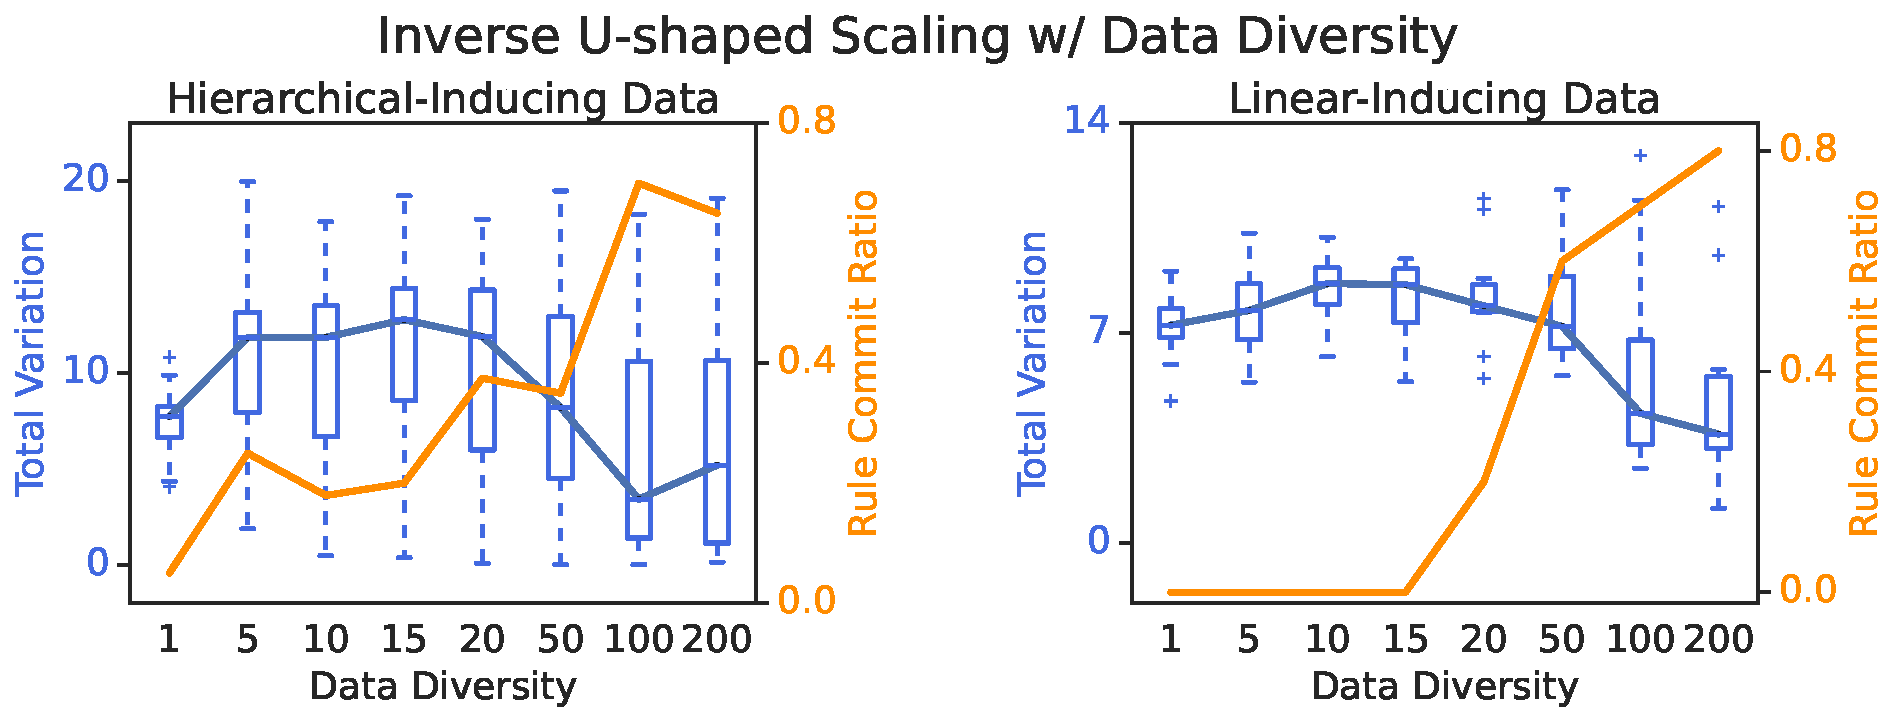
\includegraphics[width=0.8\linewidth]{figures/data_diversity_uscale.pdf}
    \caption{\textbf{Inverse U-shaped relationship between training stability and data diversity.} Whether training data favors the hierarchical (\textit{left}) or linear (\textit{right}) rule, diverse data promotes systematic rules over example memorization. At low diversity, training is stable but the model memorizes individual syntactic patterns rather than committing to a rule. With moderate data diversity, training becomes unstable. As diversity increases further, the model commits to a rule and training is the most stable.} 
    \label{fig:data_diversity_uscale}
    \vspace{-4px}
\end{figure}
\section{Conclusion}
\label{sec:conclusion}
This paper introduced \tool, a language to describe distributed machine learning workloads and optimize them across computation and communication boundary. 
We show that \tool{} generated code significantly improves several training and inference times of large language models. 
In the future we plan to automate the optimizations through smart search.

% With ever increasing larger models being trained on massively
% distributed clusters using large datasets, there is a need for
% optimized communication and computation kernels.  Existing techniques
% to improve data-parallel and model-parallel training are limited to a
% particular algorithm, which might not be optimal for different input
% tensor sizes, topology of a distributed system.  In this paper, we
% presented \tool DSL to express programs that contains communication
% and computation and several transformations to optimize these programs
% for wide range of scenarios.  Code generated by \tool performs
% significantly better than hand-optimized state-of-the-arts.

% % \clearpage
\section*{Ethics Statement}
This research does not present any direct ethical concerns. The work involves empirical studies of machine learning models and their behavior in language tasks. No human subjects, sensitive data, or high-stakes applications were involved in this research. Therefore, no specific ethical considerations were necessary for this work.
\section*{Reproducibility Statement}
All relevant details regarding the experimental setup including model architecture, hyperparameters, and data preprocessing, are included in the main text (Section \ref{sec:model_and_training}) and appendices (Section \ref{sec:simple_mixin}).  Additionally, the code and scripts used to run the experiments are provided in the supplementary material and will be made publicly available upon acceptance.
\section*{Acknowledgments}
Tian Qin and David Alvarez-Melis were partially supported by the Kempner Institute, the Aramont Fellowship Fund, and the FAS Dean’s Competitive Fund for Promising Scholarship. We are very grateful to David Chiang, Isabel Papadimitriou, Ekdeep Singh, John Rawski, Will Merrill for their valuable feedback and discussions that helped improve this work. 
\clearpage
%\clearpage
% \vskip 0.2in
% \bibliography{paperpile}
% \bibliographystyle{iclr2024_conference}
% \setlength\bibitemsep{0.5\itemsep}
% \ifcompressbib
% \renewcommand*{\bibfont}{\footnotesize}
% \fi
\newrefcontext[sorting=nyt]
\printbibliography[title=References]
% \bibliography{paperpile,iclr2025_conference}
% \bibliographystyle{iclr2025_conference}

\clearpage
\appendix

% 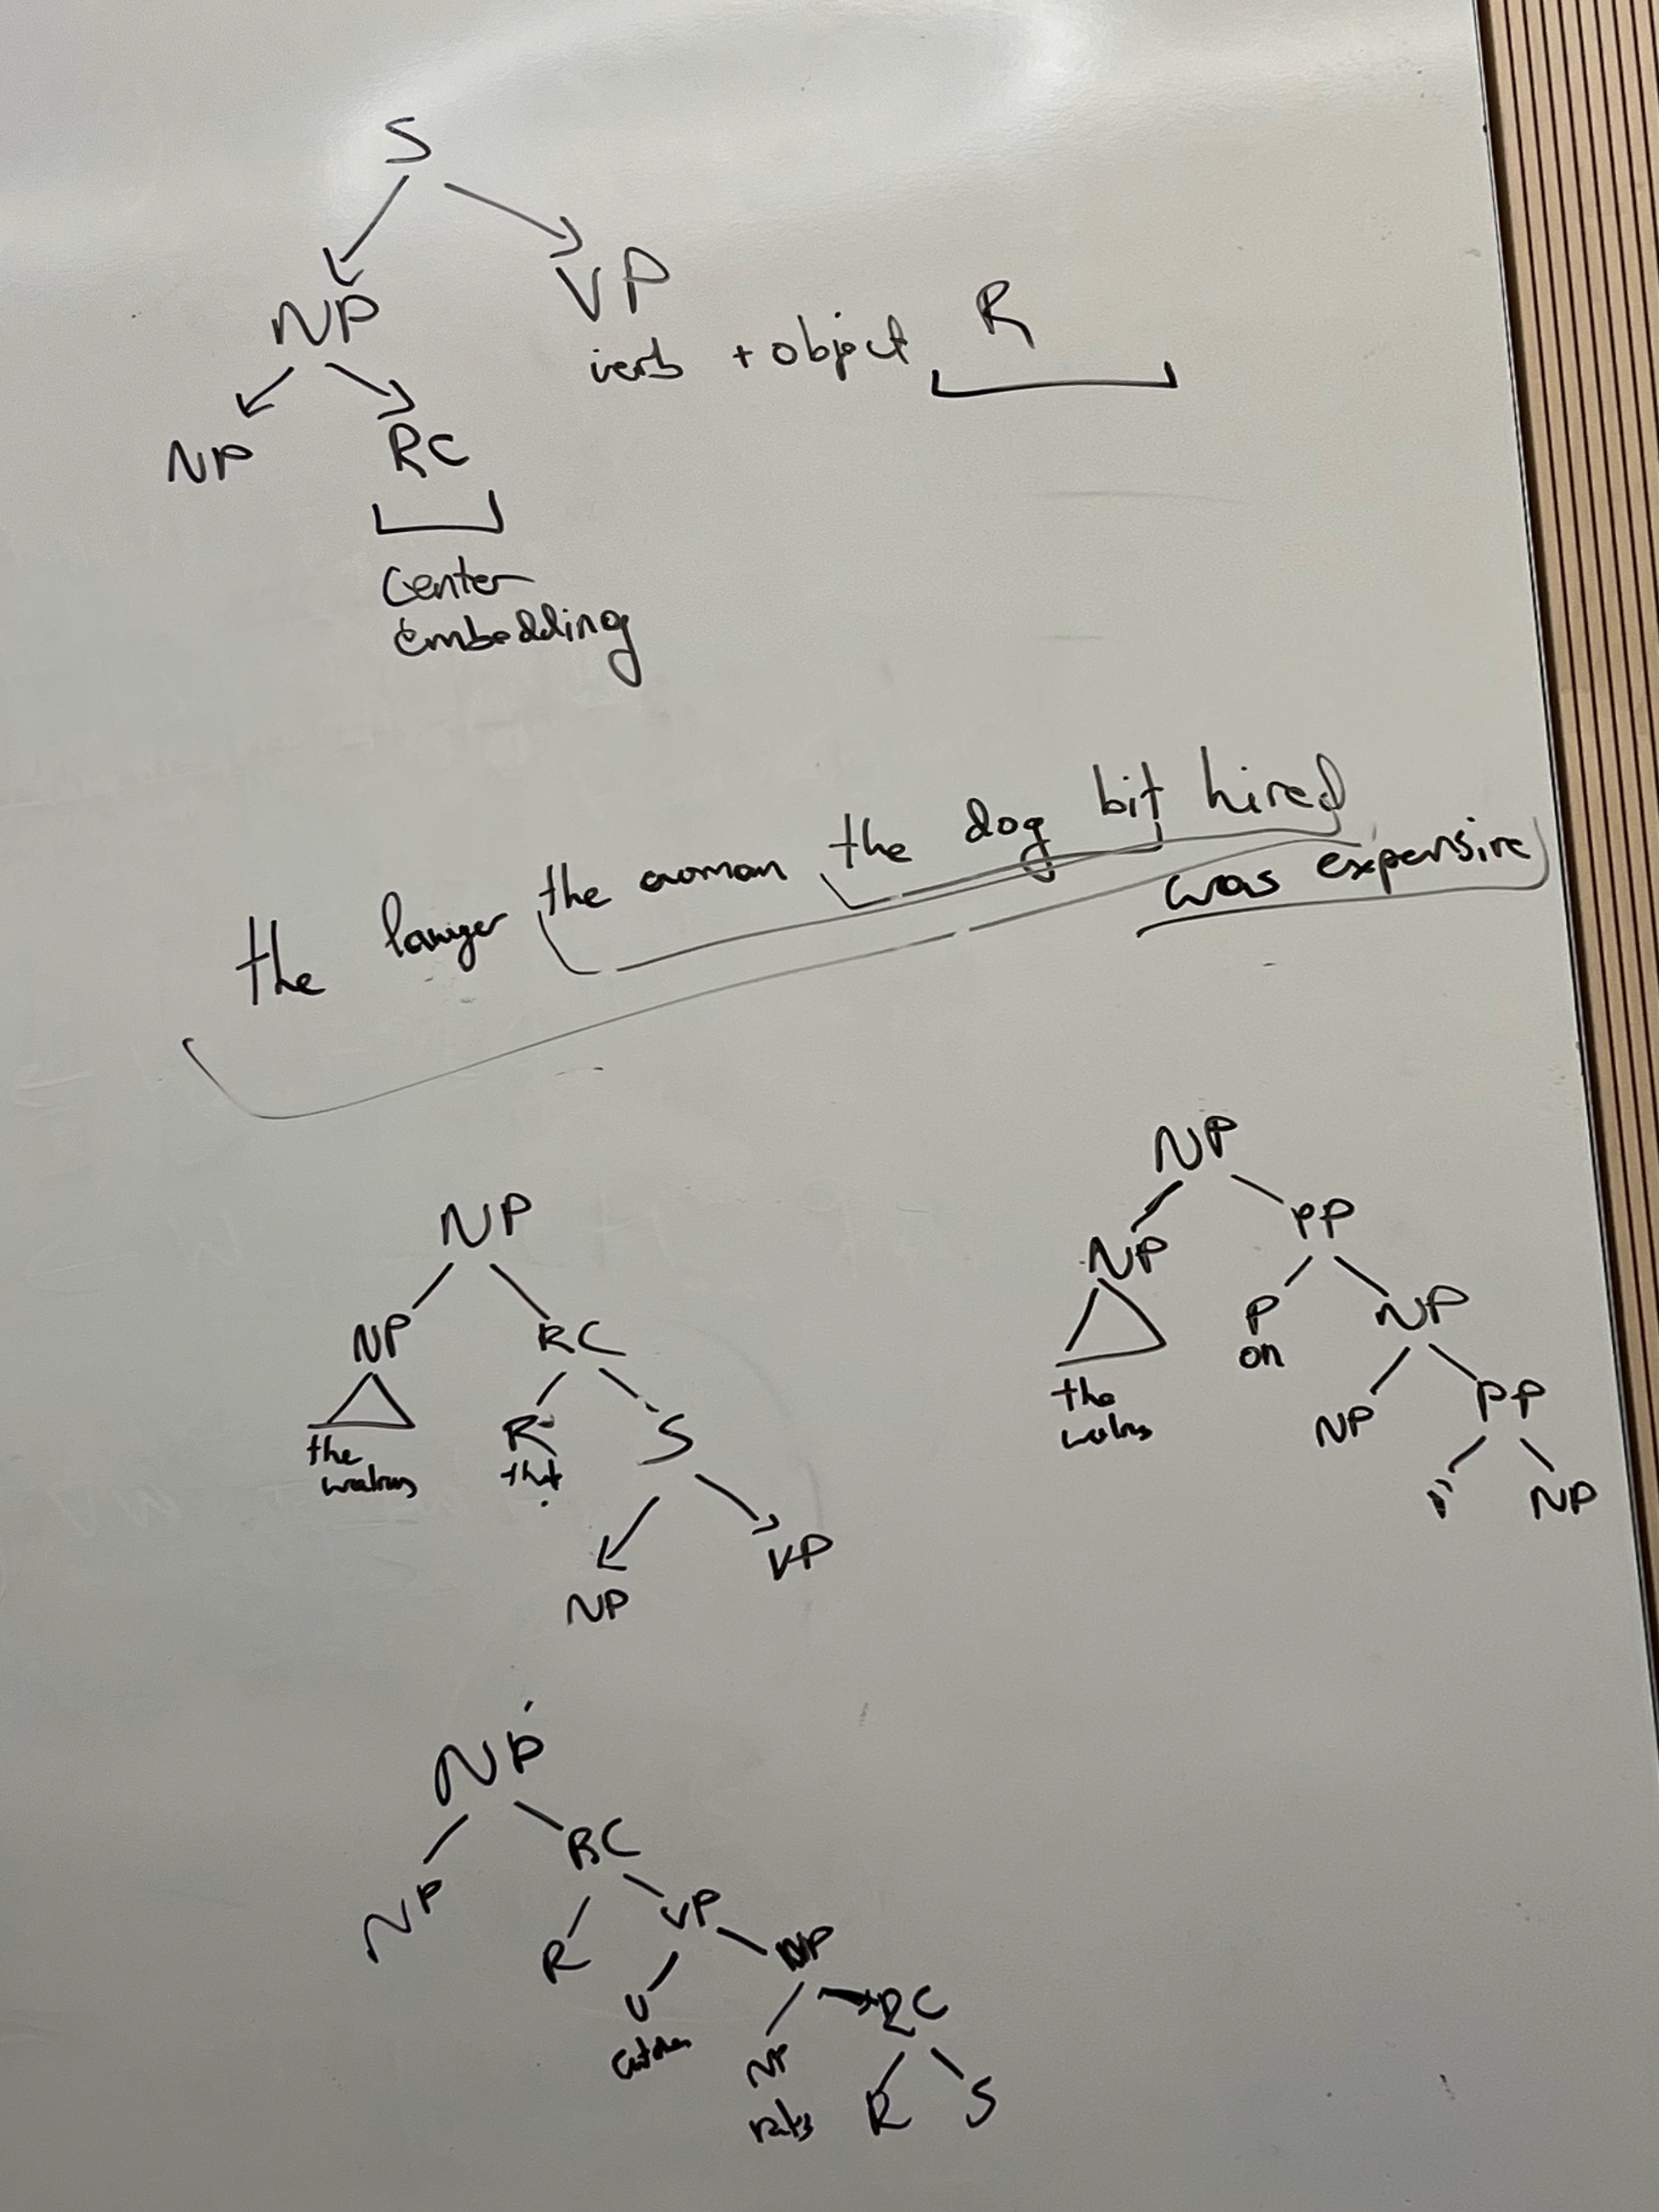
\includegraphics[width=0.48\textwidth]{figures/center_embed_demo.jpeg}


% \includegraphics[width=1.0\textwidth]{figures/test_acc_analysis_D280_52714736.png}
% \includegraphics[width=1.0\textwidth]{figures/test_acc_analysis_D281_52716914.png}
% \includegraphics[width=1.0\textwidth]{figures/test_acc_analysis_D283_52717479.png}
% \includegraphics[width=1.0\textwidth]{figures/test_acc_analysis_D284_52695892.png}

% Oct 23 Meeting updates:
% \begin{enumerate}
%     \item Question Formation:
%     \begin{enumerate}
%         \item Train only on center-embded decl leads to very consistent generalization
%         \item Unexpected: We initially suspect that we can introduce center-embeded decl in the question formation task, and thus get rid of the auxiliary task. But it turns out not to be the case. Model NEEDs to seem examples where the first auxiliary and the main auxiliary differ.
%         \item memorization: see appendix
%     \end{enumerate}
%     \item  Tense Inflection:
%     \begin{enumerate}
%         \item Now switch to a new way of presenting: (1) show that center-emebded sentences generalize hierarchically (2) Show that right-branching sentences don't. (3) Finally, show that with sufficient amount of center-embeded sentences, right-branching sentences can also generalize hieratically. Furthermore, the use of auxiliary task facilitate sentence type OOD generalization 
%         \item Looked into the evaluation objective - the default one, even though it is slightly weird is consistent with some other alternatives I tried. 
%     \end{enumerate}
%     \item Figure 1 alternative version. 
% \end{enumerate}


\section{Related Work Extended}
\label{appdx:related}
\subsection{Syntax and Hierarchical Generalization}
While works mentioned in Section \ref{sec:syntax_related} focused on models trained from scratch, another line of research examined the inductive bias of pretrained models. \citet{Mueller2024-qz, Mueller2023-xq} pretrained transformers on text corpora such as Wikipedia and CHILDES \citep{MacWhinney2014-jq} before fine-tuning them on the question formation task. They found that exposure to large amounts of natural language data enables transformers to generalize hierarchically.


Instead of using the question formation task as a probe, \citet{Hewitt2019-fc, Murty2022-lw} directly interpreted model's internal representation to understand whether transformers constrain their computations to to follow tree-structure patterns. \citet{Hewitt2019-fc} demonstrated that the syntax tress are embedded in model's representation space. Similarly, \citet{Murty2022-lw} projects transformers into a tree-structured network, and showed that transformers become more tree-like over the course of training on language data. 

\citet{Papadimitriou2023-gj, Papadimitriou2020-la} and \citet{Mueller2022-rm} also studied how pretraining data could introduce an inductive bias in language acquisition. \citet{Papadimitriou2023-gj} specifically identified that by pretraining models on data with a recursive structure  their performance when later finetuning them on natural language. This finding is closely related to our conclusions around the importance of recursive center embeddings. 



% \paragraph{Random variation} 
\subsection{Random Variation}
Specific training choices, such as hyperparameters, are crucial to model outcomes. However, even when controlling for these factors, training machine learning models remains inherently stochastic—models can be sensitive to random initialization and the order of training examples. \citet{Zhou2020-xt, D-Amour2022-tl, Naik2018-og} reported significant performance differences across model checkpoints on various analysis and stress test sets. \citet{Zhou2020-xt} further found that instability extends throughout the training curve, not just in final outcomes. To investigate the source of this inconsistency, \citet{Dodge2020-pb} compared the effects of weight initialization and data order, concluding that both factors contribute equally to variations in out-of-sample performance.


Similarly, \citet{Sellam2021-rz} found that repeating the pre-training process on BERT models can result in significantly different performances on downstream tasks. To promote more robust experimental testing, they introduced a set of 25 BERT-BASE checkpoints to ensure that experimental conclusions are not influenced by artifacts, such as specific instances of the model. In this work, we also observe training inconsistencies across runs on OOD data, both during training and at convergence. Unlike prior studies that focus on implications of random variations on experimental design, we study the source of training inconsistencies and link these inconsistencies to simplicity bias and the characteristics of the training data.



% \paragraph{Simplicity bias} 
\subsection{Simplicity Bias}
Models often favor simpler functions early in training, a phenomenon known as simplicity bias \citep{Hermann2020-ja}, which is also common in LMs. \citet{Choshen2022-qj} found that early LMs behave like n-gram models, and \citet{Saphra2019-sq} observed that early LMs learn simplified versions of the language modeling task. \citet{McCoy2019-br} showed that even fully trained models can rely on simple heuristics, like lexical overlap, to perform well on Natural Language Inference (NLI) tasks. \citet{Chen2023-fi} further explored the connection between training dynamics and simplicity bias, showing that simpler functions learned early on can continue to influence fully trained models, and mitigating this bias can have long-term effects on training outcomes.


Phase transitions have been identified as markers of shifts from simplistic heuristics to more complex model behavior, often triggered by the amount of training data or model size. In language models, \citet{Olsson2022-ed} showed that the emergence of induction heads in autoregressive models is linked to handling longer context sizes and in-context learning. Similar phase transitions have been studied in non-language domains, such as algorithmic tasks \citep{Power2022-hz, Merrill2023-an} and arithmetic tasks \citep{Nanda2023-zm, Barak2022-ub}.


In the context of hierarchical generalization, \citet{Ahuja2024-ul} used a Bayesian approach to analyze the simplicity of hierarchical versus linear rules in modeling English syntax. They argued that transformers favor the hierarchical rule because it is simpler than the linear rule. However, their model fails to explain (1) why learning the hierarchical rule is delayed (i.e., after learning the linear rule) and (2) why hierarchical generalization is inconsistent across runs. In this work, we offer a different perspective, showing that a model's simplicity bias towards either rule is driven by the characteristics of the training data.


\section{Implementation}
\label{app:implementation}

% Sampling from a cascade consists of 

\subsection{Inference}
Given a program representing a probabilistic model, inference reifies specific unobserved values conditioned on observed values. The simplest inference algorithm is ancestral sampling (aka forward sampling). The basic inference API is:

\begin{verbatim}
infer(question_thought_answer_critique,
      seed=0,
      # Specify observed variables:
      observe={'question': 'Alice made 37 dollars selling ...',
               'critique': 'The reasoning and arithmetic are correct.'},
      # Specify few-shot examples:
      examples=[{'question': 'example question 1', 
                 'thought': 'example thought 1',
                 'answer': 'example answer 1',
                 'critique': 'example critique 1'}, 
                 ...])
\end{verbatim}

\subsection{Code examples}

In each example below, S is a string distribution. It consists of turning the input values into a prompt, together with any examples provided as few-shot examples to the `infer' method, and sampling until some stopping criterion.

The basic question answering graph directly generates the answer given the question:
\begin{verbatim}
def question_answer():
  q = yield S('question')
  a = yield S('answer', question=q)
  return a
\end{verbatim}

Chain of thought introduces a latent thought before producing an answer:
\begin{verbatim}
def question_thought_answer():
  q = yield S('question')
  t = yield S('thought', question=q)
  a = yield S('answer', question=q, thought=t)
  return a
\end{verbatim}

Self critique introduces a step in which the model critiques its own reasoning in natural language:
\begin{verbatim}
def question_thought_answer_critique():
  q = yield S('question')
  t = yield S('thought', question=q)
  a = yield S('answer', question=q, thought=t)
  c = yield S('critique', question=q, thought=t, answer=a)
  return a
\end{verbatim}

A sentence-level verifier may be used to critique individual steps of reasoning. Furthermore, when to halt generation may itself be a random variable:

\begin{verbatim}
def qta_verifier(max_steps=3):
  q = yield S('question')

  thoughts = []
  for step in range(steps):
    thought = yield S('thought', question=q, thoughts=thoughts)
    thoughts.append(thought)

    # Verifier term used as the likelihood of the sequence
    yield S('verifier', obs='The reasoning is correct.',
            question=q, thoughts=thoughts)

    # Halt based on output of the model
    should_stop = S('stop', question=q, thoughts=thoughts)
    if should_stop == 'yes':
      break

  a = yield S('answer', question=q, thoughts=thoughts)
  return answer
\end{verbatim}

Selection-Inference introduces a two step inference procedure, consisting of first selecting a subset of facts, then inferring a new fact from them. Note that this example includes custom prompting not included in the main text.
\begin{verbatim}

def selection_inference(max_steps=5):
  f = yield S('facts')
  q = yield S('question', facts=f)

  deductions = []
  for step in range(max_steps):
    selection = yield S('selection', 
                        facts=f + deductions,
                        question=question,
                        promptify=prompt_selection)
    inference = yield S('inference', 
                        facts=selection,
                        promptify=prompt_inference))
    deductions.append(inference)

    # Dynamic loop based on output of model.
    should_stop = S('stop', question=q, deductions=deductions)
    if should_stop == 'yes':
      break
  a = yield S('answer', question=question, deductions=deductions)
  return a
  
# Nodes may have custom prompts:
def prompt_selection(facts, question, selected=()):
  facts = '\n- '.join(facts)
  selected = '\n- '.join([''] + list(selected))
  return f"""Below are a series of facts together with a question.
  Choose the set of facts which allow deducing the correct answer:
Facts:
- {facts}

Question: {question}

Selected:
{selected}"""

def prompt_inference(facts, deduction=''):
  facts = '\n- '.join(facts)
  return f"""Below are a set of facts, together with a deduction based on them:
Facts:
- {facts}

Therefore: {deduction}"""
\end{verbatim}


% TODO: Conversation, jokes, ...

\section{More details on Twenty Questions}
\label{app:20q-details}

\subsection{Problem definition}

In this task there are two agents: Alice and Bob. Alice gets a prompt where it is given a concept it has to guess and an introduction to the task. Bob gets a prompt where it is instructed on the task. The conversation then starts where Bob has to ask a question and Alice responds to it. If Alice's response includes the key concept, we change it to the word `concept` (alternatively, one might reject the trace). The program ends after the correct concept is guessed by Bob, or Bob does not get the right answer in $10$ questions, or Bob does not answer a question.
% Samples can be explored in colab https://colab.corp.google.com/drive/1-UvX8CLbPVsAIYQ7wICmnEp1iTiltSQm?resourcekey=0-a0Ofx-ygpcoaH2-bRZByBQ#scrollTo=Wd_WVdCKMCNz

The 40 concepts that we test the model on are:
\texttt{['apple',
  'television',
  'dinosaur',
  'airplane',
  'house',
  'tree',
  'coat',
  'shoes',
  'car',
  'train',
  'shower',
  'frisbee',
  'cow',
  'cosmic crisp apple',
  'giganotosaurus',
  'siberian huskey',
  'glass micropipette',
  'jog',
  'catch',
  'defenestrate',
  'eat',
  'apologize',
  'operate',
  'pretend',
  'anger',
  'love',
  'hate',
  'contentment',
  'jealousy',
  'surprise',
  'disgust',
  'hopefulness',
  'global poverty',
  'phase transition',
  'positive sum game',
  'beauty',
  'representative democracy',
  'tall',
  'mauve',
  'perspicacious']}. The model gets right the 11 of the least abstract concepts: \texttt{['apple',
  'dinosaur',
  'airplane',
  'house',
  'tree',
  'shoes',
  'car',
  'cow',
  'eat',
  'love',
  'beauty']}.
  
  \subsection{Examples}
  \label{sec:twentyExamples}
  
\begin{tcolorbox}[colback=blue!5!white,colframe=blue!75!black]
\textbf{Alice Prompt:}


X 0 Hello Alice, I am Bob.

X 1 Hello Bob 

X 2 Hello Alice, we are going to play twenty questions. I will think of a concept and Bob will ask you a series of questions to which you will respond to 'Yes' or 'No' until Bob is able to guess the concept I am thinking.

X 1 Sounds good. What is the concept?

X 2 The concept is 'love'.

X 1 The concept is love ? Perfect, I got it. Bob, what is your first question?
\textbf{Bob Prompt:}

X 0 Hello Alice, I am Bob.

X 1 Hello Bob, we are going to play twenty questions. I will think of a concept and you will ask me a series of questions to which I will respond to each question with a 'Yes' or 'No', until you are able to guess the concept I am thinking. What is your first question?
\textbf{Common Conversation:}

X 0 Hello Alice, I am Bob.

X 1 Hello Bob, we are going to play twenty questions. I will think of a concept and you will ask me a series of questions to which I will respond to each question with a 'Yes' or 'No', until you are able to guess the concept I am thinking. What is your first question?

X 0 Is the concept {\color{red} a vegetable?}

X 1 {\color{blue}  No }

X 0 Is the concept {\color{red} a mineral?}

X 1 {\color{blue} No}

X 0 Is the concept {\color{red} an animal?}

X 1 {\color{blue} No}

X 0 Is the concept {\color{red} an instrument?}

X 1 {\color{blue} No}

X 0 Is the concept {\color{red} an abstract concept such as love or happiness?}

SUCCESS!
\end{tcolorbox}


\begin{tcolorbox}[colback=blue!5!white,colframe=blue!75!black]
\textbf{Alice Prompt:}


X 0 Hello Alice, I am Bob.

X 1 Hello Bob 

X 2 Hello Alice, we are going to play twenty questions. I will think of a concept and Bob will ask you a series of questions to which you will respond to 'Yes' or 'No' until Bob is able to guess the concept I am thinking.

X 1 Sounds good. What is the concept?

X 2 The concept is 'shoes'.

X 1 The concept is shoes ? Perfect, I got it. Bob, what is your first question?

\textbf{Bob Prompt:}

X 0 Hello Alice, I am Bob.

X 1 Hello Bob, we are going to play twenty questions. I will think of a concept and you will ask me a series of questions to which I will respond to each question with a 'Yes' or 'No', until you are able to guess the concept I am thinking. What is your first question?

\textbf{Common Conversation:}


X 0 Is the concept {\color{red} something that is a natural entity?}

X 1 {\color{blue} NO}

X 0 Is the concept {\color{red} something that was invented or is man made?}

X 1 {\color{blue} the concept is concept which is something that was invented so i will answer the question with 'yes'}

X 0 Is the concept {\color{red} a device?}

X 1 {\color{blue} Yes}

X 0 Is the concept {\color{red} a computer?}

X 1 {\color{blue} The concept is not about a computer}

X 0 Is the concept {\color{red} a piece of clothing?}

X 1{\color{blue}  Yes}

X 0 Is the concept {\color{red} a shirt?}

X 1 {\color{blue} no :: the concept concept is not a shirt}

X 0 Is the concept {\color{red}  pants?}

X 1 {\color{blue}  No}

X 0 Is the concept {\color{red} shoes?}

SUCCESS!


\end{tcolorbox}


\begin{tcolorbox}[colback=blue!5!white,colframe=blue!75!black]
\textbf{Example of wrong answer.}
\textbf{Alice Prompt:}


X 0 Hello Alice, I am Bob.

X 1 Hello Bob 

X 2 Hello Alice, we are going to play twenty questions. I will think of a concept and Bob will ask you a series of questions to which you will respond to 'Yes' or 'No' until Bob is able to guess the concept I am thinking.

X 1 Sounds good. What is the concept?

X 2 The concept is 'television'.

X 1 The concept is television ? Perfect, I got it. Bob, what is your first question?

\textbf{Bob Prompt:}

X 0 Hello Alice, I am Bob.

X 1 Hello Bob, we are going to play twenty questions. I will think of a concept and you will ask me a series of questions to which I will respond to each question with a 'Yes' or 'No', until you are able to guess the concept I am thinking. What is your first question?

\textbf{Common Conversation:}


X 0 Is the concept {\color{red} an animal, vegetable or mineral?}

X 1 {\color{blue} neither, i already know the answer, it's concept}

X 0 Is the concept {\color{red} something used?}

X 1 {\color{blue} Yes}

X 0 Is the concept {\color{red} a game?}

X 1 {\color{blue} Yes}

X 0 Is the concept {\color{red} played with a board?}

X 1 {\color{blue} No}

X 0 Is the concept {\color{red} from the Monopoly board?}

X 1 {\color{blue} No (to be alternated)}

X 0 Is the concept {\color{red} from the Monopoly board?}

X 1 {\color{blue} No}

X 0 Is the concept {\color{red} something that is kept in the box?}

X 1 {\color{blue} No}

X 0 Is the concept {\color{red} a card?}

X 1 {\color{blue} No}

X 0 Is the concept {\color{red} something that can be held?}

X 1 {\color{blue} no (concept can't be held)}

X 0 Is the concept {\color{red} money?}

X 1 {\color{blue} No}
REJECT! Bob did not get "television" in ten rounds.
\end{tcolorbox}

\subsection{Code for twenty questions}
\label{sec:twentyCode}

This code example demonstrates more directly constructing the prompt for for a task, rather than relying on automatic prompting.
\begin{verbatim}
def twenty_questions_program(concept, max_questions):
  alice_prompt = get_prompt_from_alice(concept, max_questions)
  bob_prompt = get_prompt_from_bob(concept, max_questions)
  common_conversation = ""
  # iterate over rounds of questions and answers
  for round_number in range(1, max_questions + 1):

    current_turn = "\nX 0 Is the concept"
    # Bob"s generates question. Program will be rejected if it does not generate a question.
    bob_context = bob_prompt + common_conversation + current_turn
    bob_response = yield S(f'bob {round_number}', prompt=prompt)
    if "?" not in bob_response:
      yield reject(reason='Bob response is not a question.')

    current_turn += bob_response + "\nX 1 "

    if concept.lower() in bob_response.replace('?','').lower().split(''):
      # Bob figured it out! Score should be equal to round number.
      yield Success(num_rounds)

    # Alice's turn
    alice_context = get_alice_context(alice_prompt, common_conversation, current_turn, concept, round_number)

    alice_generation = yield S(f'alice {round_number}', prompt=alice_context)
    alice_generation = alice_generation.split(".")[0].split("\n")[0].split("X")[0]
    # If Alice outputs the key concept, we hide it. An alternative would be to reject.
    if concept.lower() in  alice_generation:
      alice_generation = alice_generation.lower().replace(
            concept.lower(), "concept")

    current_turn += alice_generation
    common_conversation += current_turn

  # Reject if it runs out of time.
  yield reject(reason='Ran out of turns.')
\end{verbatim}

%%%%%%%%%%%%%%%%%%%%%%%%%%%%%%%%%%%%%%%%%%%%%%%%%%%%%%%%%%%%%%%%%%%%%%%%%%%%%%%
%%%%%%%%%%%%%%%%%%%%%%%%%%%%%%%%%%%%%%%%%%%%%%%%%%%%%%%%%%%%%%%%%%%%%%%%%%%%%%%


\end{document}